\documentclass[border=8pt]{standalone}
\usepackage[utf8]{inputenc}
\usepackage{tikz}
\usetikzlibrary{positioning}

\tikzset{
  debole/.style = {rectangle, draw, thick, fill=blue!8, double, double distance=1.5pt, minimum width=28mm, minimum height=16mm, font=\small},
  attr/.style   = {circle, draw, thick, fill=white, minimum size=5pt, inner sep=0},
  pk/.style     = {circle, draw, thick, fill=black, minimum size=5pt, inner sep=0},
  link/.style   = {thick},
  et/.style     = {font=\footnotesize}
}

\begin{document}
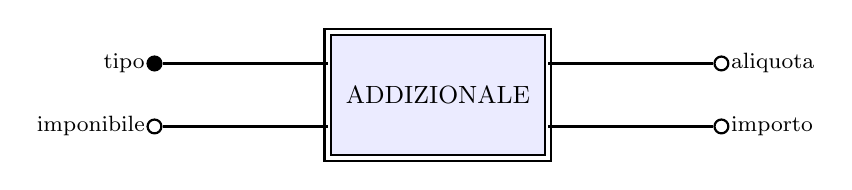
\begin{tikzpicture}
  \node[debole] (E) {ADDIZIONALE};
  \node[pk]   (t)  at (-3.6, 0.4){}; \draw[link] (-1.4, 0.4)--(t);  \node[et,left] at (t)  {tipo};
  \node[attr] (im) at (-3.6,-0.4){}; \draw[link] (-1.4,-0.4)--(im); \node[et,left] at (im) {imponibile};
  \node[attr] (al) at ( 3.6, 0.4){}; \draw[link] ( 1.4, 0.4)--(al); \node[et,right] at (al) {aliquota};
  \node[attr] (imp) at ( 3.6,-0.4){}; \draw[link] ( 1.4,-0.4)--(imp); \node[et,right] at (imp) {importo};
\end{tikzpicture}
\end{document}
